\subsection{Input Constrained and Soft Output Constrained MPC - Closed Loop Simulation}
In this section the hard input and soft output constrained MPC is simulated on both the linear and non-linear system. For this simulation, the tuning is set as:
\begin{equation}
    \begin{gathered}
        W_z=100 \quad W_u=0 \quad W_{du}=0\\
        W_{t1}=10000 \quad W_{t2}=10000 \quad W_{s1}=10000 \quad W_{s2}=10000
    \end{gathered}
\end{equation}
The constraints is set to 
\begin{equation}
    u_{min}=0\quad u_{max}=450\quad \Delta u_{min}=-10\quad \Delta u_{max}=10 \quad Z_{min} = \begin{bmatrix} 85 \\ 105 \end{bmatrix} \quad Z_{max} = \begin{bmatrix} 110 \\ 120 \end{bmatrix}
\end{equation}
It should be noticed that the values shown in the plot is absolute values.
\begin{figure}[H]
    \centering
    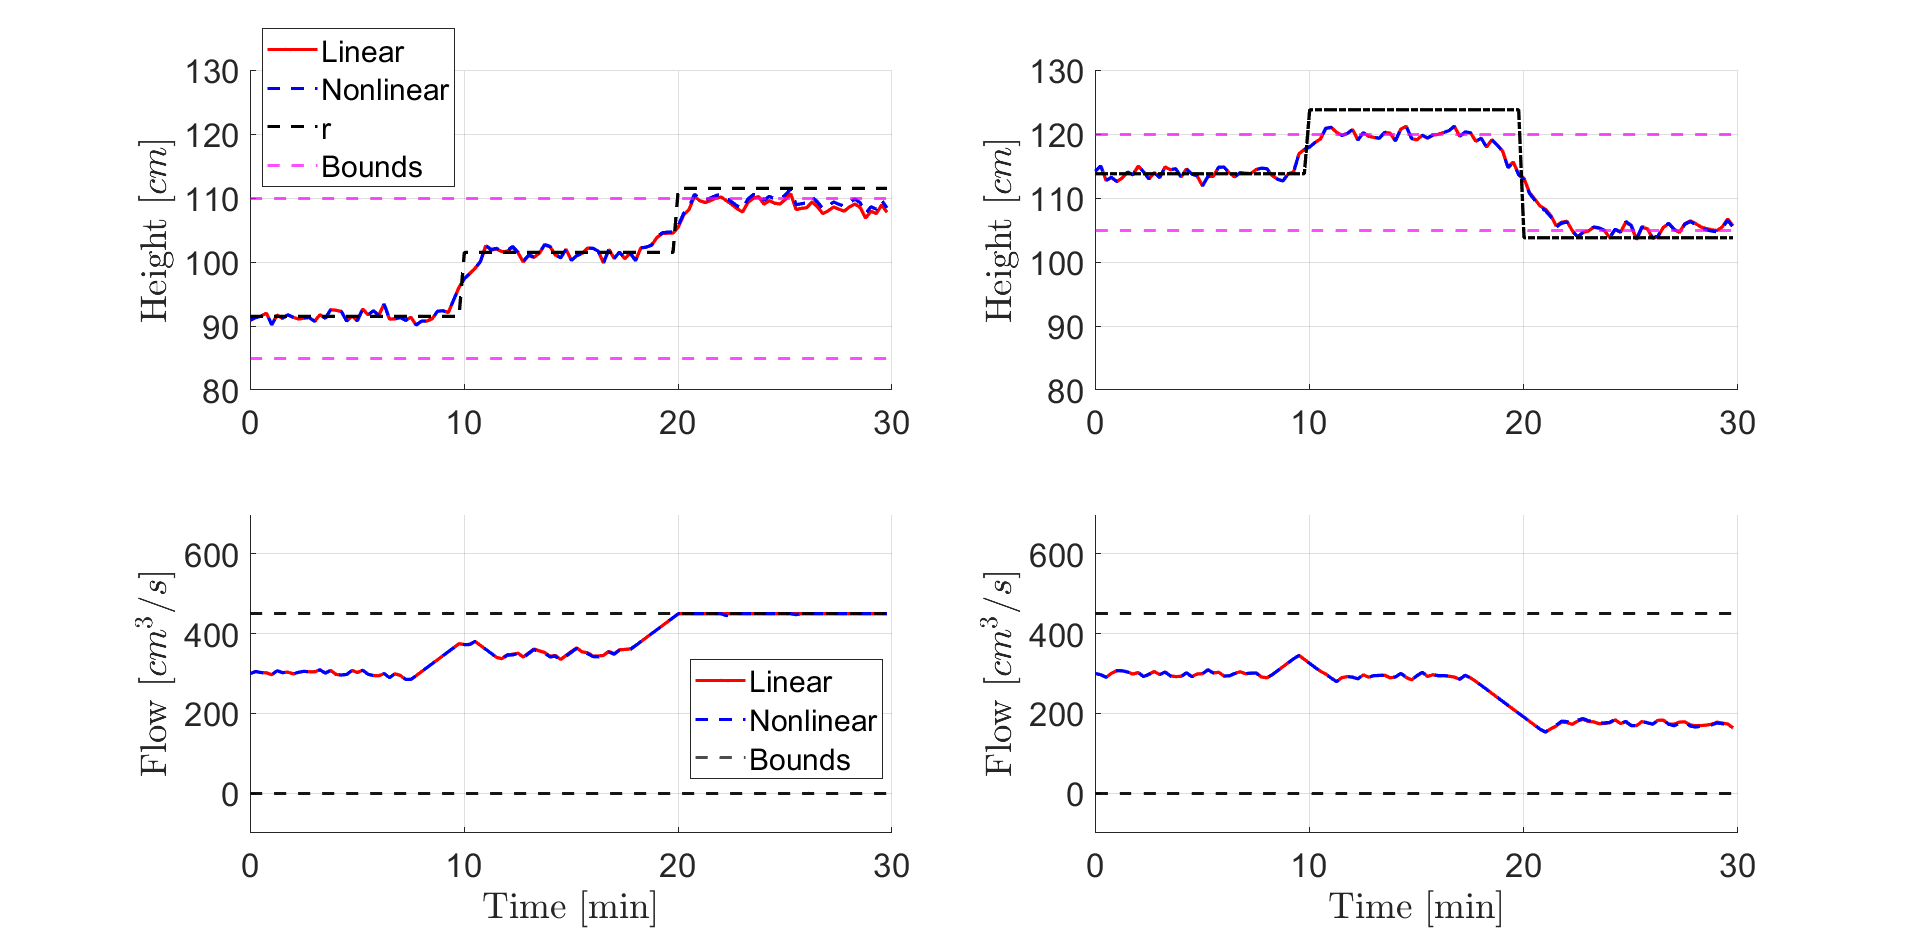
\includegraphics[width=1\textwidth]{Figures/Pr10.3_InOut_con_MPC.png}
    \caption{Input constrained output constrained MPC - Simulation on linear and non-linear model}
    %\label{fig:Kalman_stoc_state_step}
\end{figure}
By first analyzing the output in tank 1, it is seen that at $T=20\,[min]$ the reference changes. The system is both limited by the input which is a hard constraint, and therefore the system is not able to reach desired output. For tank 2, the input constraints are far from the operation, so these will not limit the system. The output constraint is clearly seen from $T=10-20\,[min]$ where the output is limited. The idea of a soft constraint is clearly seen since the controller allows system to trespass the value (which is caused by the present of noise). At $T=20\,[min]$ the reference changes again, and here the lower output constraint limits the output. Once again, the presence of noise is causing the output to become lower than the limit in some small periods. \\
Due to the structure of the system, the output constraint on e.g. tank 2 can also affect tank 1. If the water level reached the constraint, this will limit the flow input. But since the flow from the pump affects both tanks, the dynamics in tank 1 can be affected.